\pgfsetplotmarksize{0pt}
\begin{figure}
 \centering
 \caption{\label{fl_conv0}FLClustered/test0.txt},
 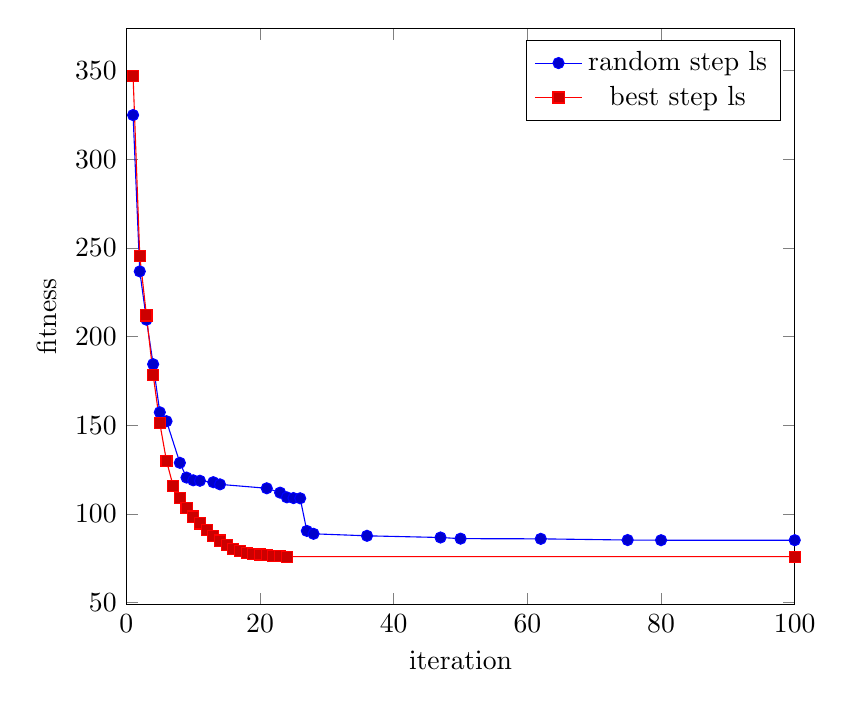
\begin{tikzpicture}
 \begin{axis}[
   width=0.7\textwidth,
   scale only axis,
   xlabel=iteration,
   ylabel=fitness,
   xmin=0,xmax=100,
   domain=0:100]
   \addplot coordinates {
     (0,inf)
     (1,324.942)
     (2,236.782)
     (3,209.541)
     (4,184.435)
     (5,157.321)
     (6,152.289)
     (8,128.823)
     (9,120.497)
     (10,118.965)
     (11,118.708)
     (13,117.899)
     (14,116.674)
     (21,114.465)
     (23,112.007)
     (24,109.374)
     (25,108.944)
     (26,108.819)
     (27,90.4234)
     (28,88.7929)
     (36,87.6585)
     (47,86.7098)
     (50,86.0617)
     (62,85.9504)
     (75,85.279)
     (80,85.1812)
     (100,85.1812)
   };
   \addlegendentry{random step ls}
   \addplot coordinates {
     (0,inf)
     (1,346.828)
     (2,245.422)
     (3,211.931)
     (4,178.561)
     (5,151.073)
     (6,129.859)
     (7,115.752)
     (8,108.788)
     (9,103.321)
     (10,98.5095)
     (11,94.646)
     (12,90.7951)
     (13,87.4437)
     (14,84.9935)
     (15,82.5473)
     (16,80.3739)
     (17,78.9966)
     (18,78.1543)
     (19,77.4955)
     (20,77.1273)
     (21,76.7786)
     (22,76.46)
     (23,76.0552)
     (24,75.926)
     (100,75.926)
   };
   \addlegendentry{best step ls}
 \end{axis}
 \end{tikzpicture}
\end{figure}
